\chapter{Génération de la liste des oSoP à partir du SIF}

La forme implicite spécialisée aka S.I.F\footnote{Specialized Implicite Form} permet de représenter efficacement un filtre linéaire. Pour l'implémenter réellement, il faut choisir la nature de la cible : logicielle ou matérielle. [Thèse Benoit]


Dans le cas de l'implémentation logicielle, la taille des variables, constantes et opérateurs est fixée par la cible. 
Par contre, pour l'implémentation matérielle, les largeurs peuvent varier selon la plage des valeurs que peuvent contenir chaque variable ainsi que la précision voulue. C'est ce qu'on appelle le paradigme des largeurs multiples. ( Voir Benoit page 146 : Optimisation des largeurs )
[ Voir aussi page 166 : implémentation HW]


\section{La représentation en Espace d'État équivalent au SIF}
\subsection{la représentation d'état}
Il y a plusieurs manière de décrire un système dynamique. La représentation d'état est une modélisation sous forme matricielle en utilisant des variables d'état... Pour notre cas, on a une représentation discrète et linéaire.
[Equation + légende + petite explication]

\subsection{Déduction du State-Space équivalente}
[Equation du SIF + nom des équations ]
%\begin{equation}
\begin{align*}
J.t(k+1) &= \qquad \qquad \quad M.x(k) + N.u(k) \\
x(k+1) &= K.t(k+1) + P.x(k) + Q.u(k) \\
y(k) &= L.t(k+1) + R.x(k) + S.u(k)
\end{align*}
%\end{equation}
Le principe consiste à intégrer les calculs intermédiaires dans l'équation d'état et de sortie. 

\begin{align*}
[calculs] \\
\smallskip
A &= K.J^{-1}.M + P \\
B &= K.J^{-1}.N + Q \\
C &= L.J^{-1}.M + R \\
D &= L.J^{-1}.N + S
\end{align*}

\section{Calcul de Hu}
La fonction de transfert Hu sert à évaluer quel effet a l'entrée sur les variables .
\begin{figure}[h]
\centering
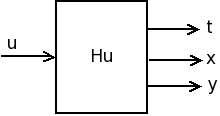
\includegraphics[scale=0.5]{Hu}
\caption{La fonction de transfert Hu}
\end{figure}

\bigskip
Pour le calculer, on part toujours du S.I.F qui décrit notre système.

[ Equations ]

\section{Calcul de He}
He sert à voir l'effet des erreurs accumulées par les variables sur la sortie.
\begin{figure}[h]
\centering
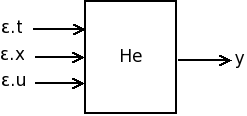
\includegraphics[scale=0.5]{He}
\caption{La fonction de transfert He}
\end{figure}

\section{Calcul de DC-Gain pour un State-Space}
Le DC-G est le gain en mode statique ou la fréquence du signal est nulle.
Le gain DC-G en temps discret est la valeur de la fonction de transfert lorsque $z=1$ \\
Pour les modèles en représentation d'états avec les matrices $(A, B, C, D)$ : \\
$G_{DC} = D + C.(I-A)^{-1}.B$

\section{Calcul du WCPG - Worst Case Peak Gain - pour un State-Space}
Le W.C.P.G est la plus grande valeur de la sortie pour toute valeur possible de l'entrée.
Pour un système modélisé dans la représentation d'états, on a le définit comme suit : \\ 
$$WCPG = |D|  + \sum_{k=0}^{\infty} |C.A^{k}.B|$$

